\section{Teil 2: Wellenlänge}
  In diesem Versuchsteil gilt es die genaue Wellenlänge der Cadmium-Linie zu bestimmen, Wir nutzen dazu zunächst das Spektrum einer Neon-Lampe als Referenz.
  Wir bestimmen wie zuvor mit \textbf{JImage} und \textbf{Python} die Position der Linien mit Hilfe eines Gauss-Fits.

  Das aufgenommene Spektrum sowohl der Neon-, als auch der Cadmium-Lampe sind in \hyperref[plt::5]{Abb. \ref*{plt::5}} zu sehen, für welches die folgenden Referenzwerte genutzt werden:
  \begin{align}
    \lambda_{Ne,1} = \SI{633.443}{\nano\metre}\nonumber\\
    \lambda_{Ne,2} = \SI{638.299}{\nano\metre}\nonumber\\
    \lambda_{Ne,3} = \SI{640.225}{\nano\metre}\nonumber\\
    \lambda_{Ne,4} = \SI{650.623}{\nano\metre}\nonumber\\
    \lambda_{Ne,5} = \SI{653.288}{\nano\metre}\nonumber\\
    \lambda_{Ne,6} = \SI{659.895}{\nano\metre}
  \end{align}


  \begin{figure}[H]
    \centering
    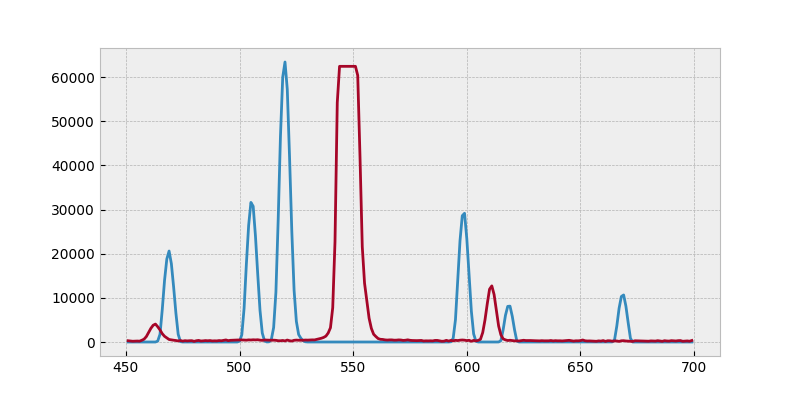
\includegraphics[width=\textwidth]{Auswertung/wavelength_analysis/wl}
    \caption{Cadmium- (Rot) und Neon- (Blau) Linien, y-Achse arbiträr}
    \label{plt::5}
  \end{figure}

  \subsection{Cadmium-Linie}
    Aus den so bestimmten Werten ergibt sich der folgende Zusammenhang (\hyperref[plt::6]{Abb. \ref*{plt::6}}), für Position und Wellenlänge, sowie die Wellenlänge der Cadmium-Linie.
    \begin{align}
      a_{Cd}       &= \SI{547.945+-4.310}{px}\\
      \lambda_{Cd} &= \lambdaCd \label{val::lcd}
      \intertext{mit dem Theoriewert}
      \lambda_{Cd,theo} &= \lambdaCdTheo
    \end{align}
    und einer Abweichung von \SI{.14}{\sigma}

    \subsection{unbekannte Linie}
      In unserem Spektrum sollte sich eine weitere Linie befinden, welche bei etwa $\SI{652}{\nano\metre}$ zu erkennen sei. diese liegt bei uns bei
      \begin{align}
        \lambda_{uk} = \lambdaUk
      \end{align}
      was nach \cite{nist.gov.uk}, entweder mit Thorium oder Xenon übereinstimmt
      \begin{align}
        \lambda_{Th I, L5951} = \lambdaTh\\
        \lambda_{Xe I, L7292} = \lambdaXe
      \end{align}
      Wir nehmen an, dass es sich hierbei um Xenon handelt, da dieses gasförmig und nichtmetallisch ist.

    \begin{landscape}
      \thispagestyle{empty}
      \begin{figure}
        \vspace*{-2cm}
        \caption{Zusammenhang zwischen Position und Wellenlänge in unseren Beobachtungen}
        \hspace*{-6cm}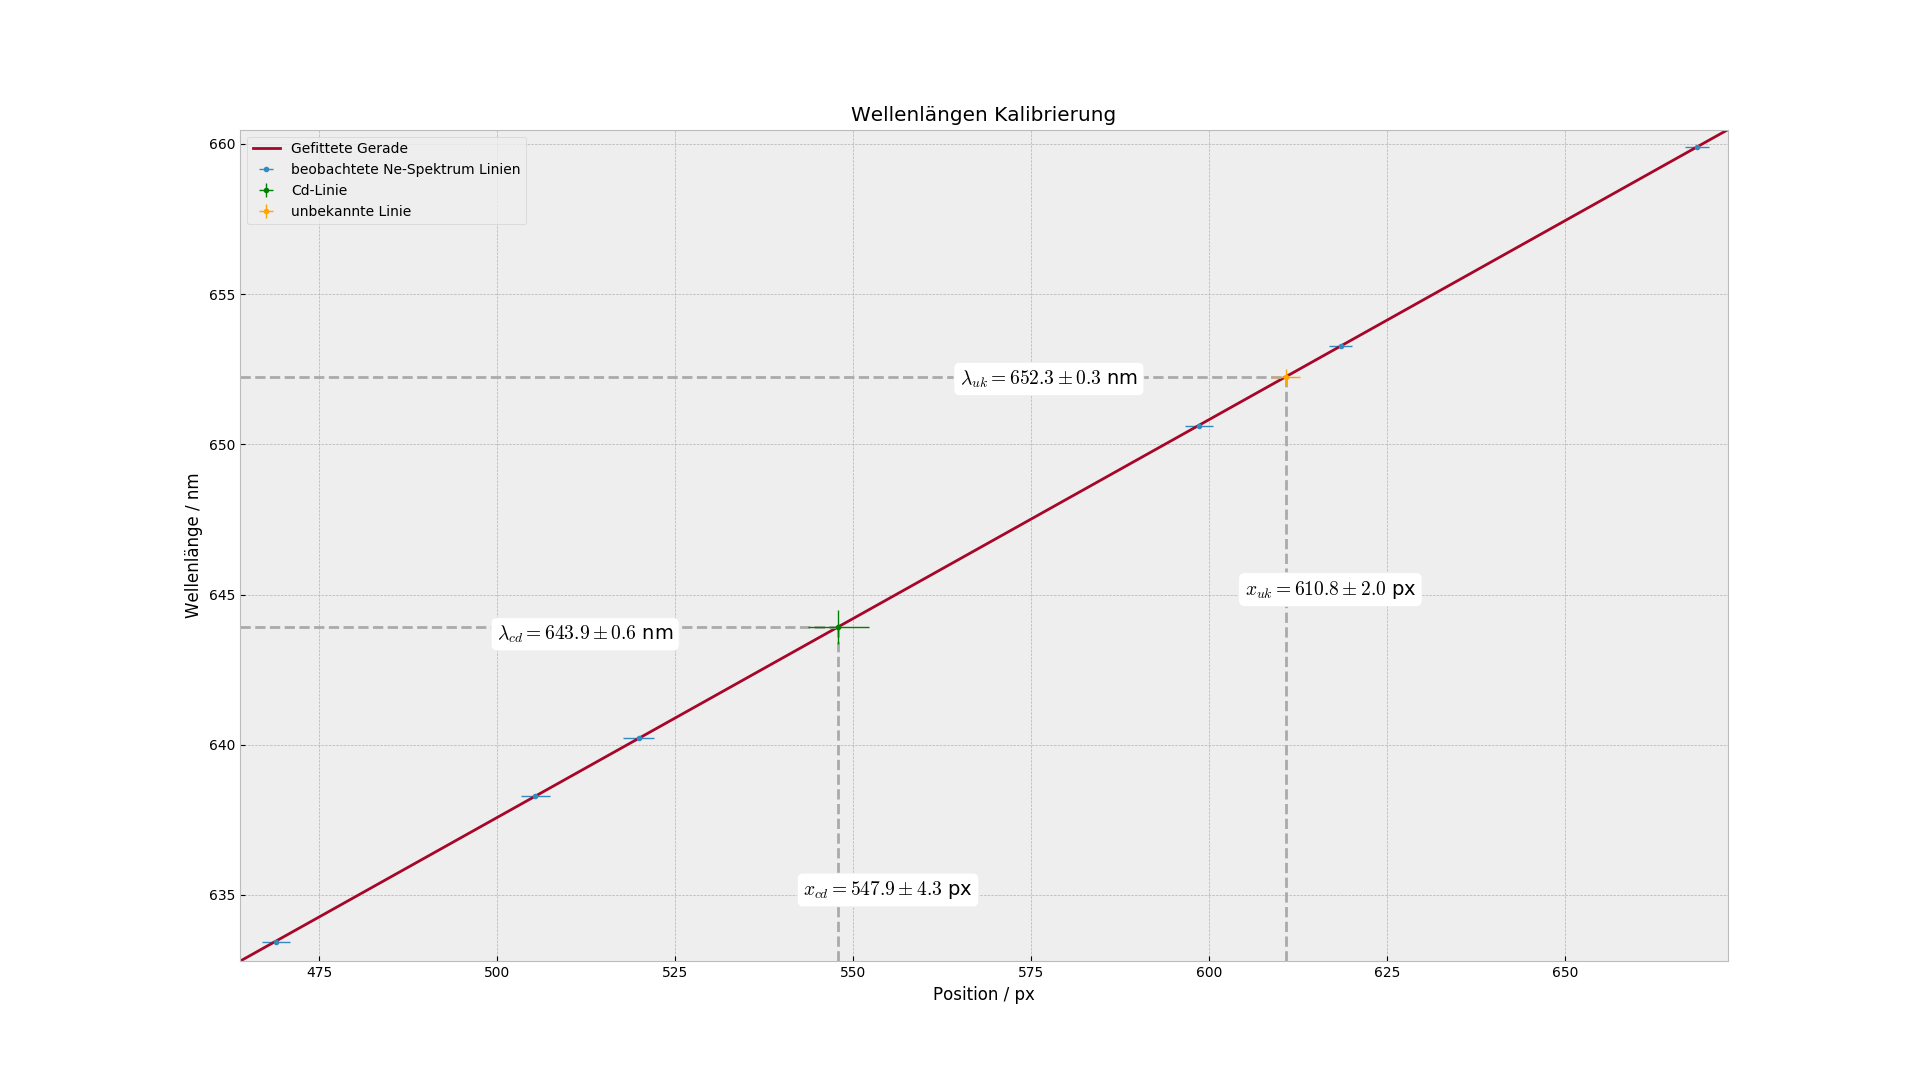
\includegraphics[width=1.5\paperwidth]{Auswertung/wavelength_analysis/wl_ne_cal}
        \label{plt::6}
      \end{figure}
    \end{landscape}
